With the \ommt translation of formal libraries, the originating systems gain access to library management
facilities implemented at the \ommt level.\footnote{The description of services in this Section has been adapted from \cite{KohMueOwr:mpagsiuf17} and \cite{ConKohMue:rdaml19}}  There are two ways to exploit this: publishing the converted libraries on a dedicated server, like the \mathhub system~\cite{MathHub:on}, or running the \omdoc/\mmt toolstack locally. Both options offer similar functionality, the main
difference is the intended audience: the first option is for outside users who want to
access the libraries, and the latter is for users who develop new
content or refactor the library.

\mathhub (see \autoref{sec:intro:mathhub}) bundles a GitLab-based repository
manager with \mmt and various periphery systems into a common, web-based user
interface. We commit the exported libraries -- exemplarily from \pvs -- as \ommt files into a
repository to make these available via the
\begin{inparaenum}[\em i\rm)]
\item \mathhub user interface,
\item \mmt presentation web server,
\item \mmt web services, and 
\item the \mws daemon.
\end{inparaenum}
All of these components give the user different ways of interacting with the system and
content. Below we explore three examples that are directly useful for \pvs users, but the
services apply similarly to users of other systems.\medskip

The local workflow installs \ommt tools on the same machine as \pvs.
In that case, users are able to browse the current version of the available \pvs libraries
including all experimental or private theories that are part of the current development.
This also enables PVS to use \ommt services as background tools that remain transparent to the PVS user.

\begin{figure}[ht]\centering
  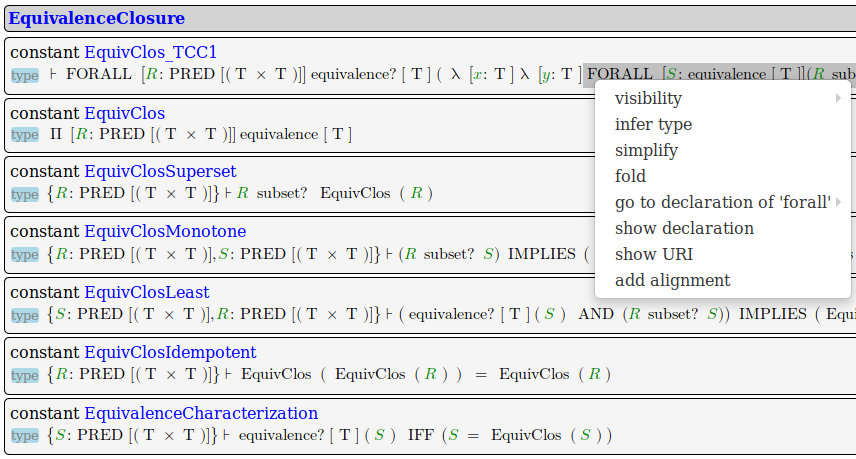
\includegraphics[width=\textwidth]{img/pvs-mathhub}
  \caption{The PVS Prelude in the \mmt Browser}\label{fig:screenshot1}
\end{figure}

In both workflows, \ommt-based periphery systems become available to the PVS user that are
either not provided by the PVS tools or in a much restricted way. We will go over the
three most important ones in detail.

\subsection{Browsing and Interaction}
 
The transformed PVS content can be browsed interactively in the document-oriented \mathhub
presentation pages (theories as active documents) and in the \mmt web browser (see
\autoref{fig:screenshot1}). Both allow interaction with the PVS content via a generic
Javascript-based interface. This provides buttons to toggle the visibility of parts
computed by PVS -- e.g. omitted types and definitions -- at the declaration level. The
right-click menu shown in \autoref{fig:screenshot1} is specific to the selected
sub-formula (highlighted in gray); here we have eight applicable interactions which range
from inferring the subformula type via definition lookup to management actions such as
registering an alignment to concepts in other libraries. New interactions can be added as
they become available in the MMT system.

The \mmt instance in the local workflow provides the additional feature of inter-process
communication between PVS and \mmt as a new menu item: the action \emph{navigate to this
  declaration in connected systems}.  Florian Rabe implemented a listener for this action that
forwards the command to PVS via an XML-RPC call at the default PVS port.  Correspondingly,
Sam Owre implemented an experimental handler in the PVS server that opens the corresponding file in the PVS emacs
system and navigates to the relevant line -- unfortunately, due to time constraints this functionality has so far not been fully developed and integrated in an official \pvs release.

\subsection{Graph Viewer}

\mathhub includes a theory graph viewer developed by Marcel Rupprecht that allows interactive, web-based exploration of
the \ommt theory graphs~\cite{RupKohMue:fitgv17}. It builds on the \texttt{visjs} JavaScript visualization
library~\cite{visjs:on}, which uses the HTML5 canvas to layout and interact with graphs
client-side in the browser.

\begin{figure}[ht]\centering
  \fbox{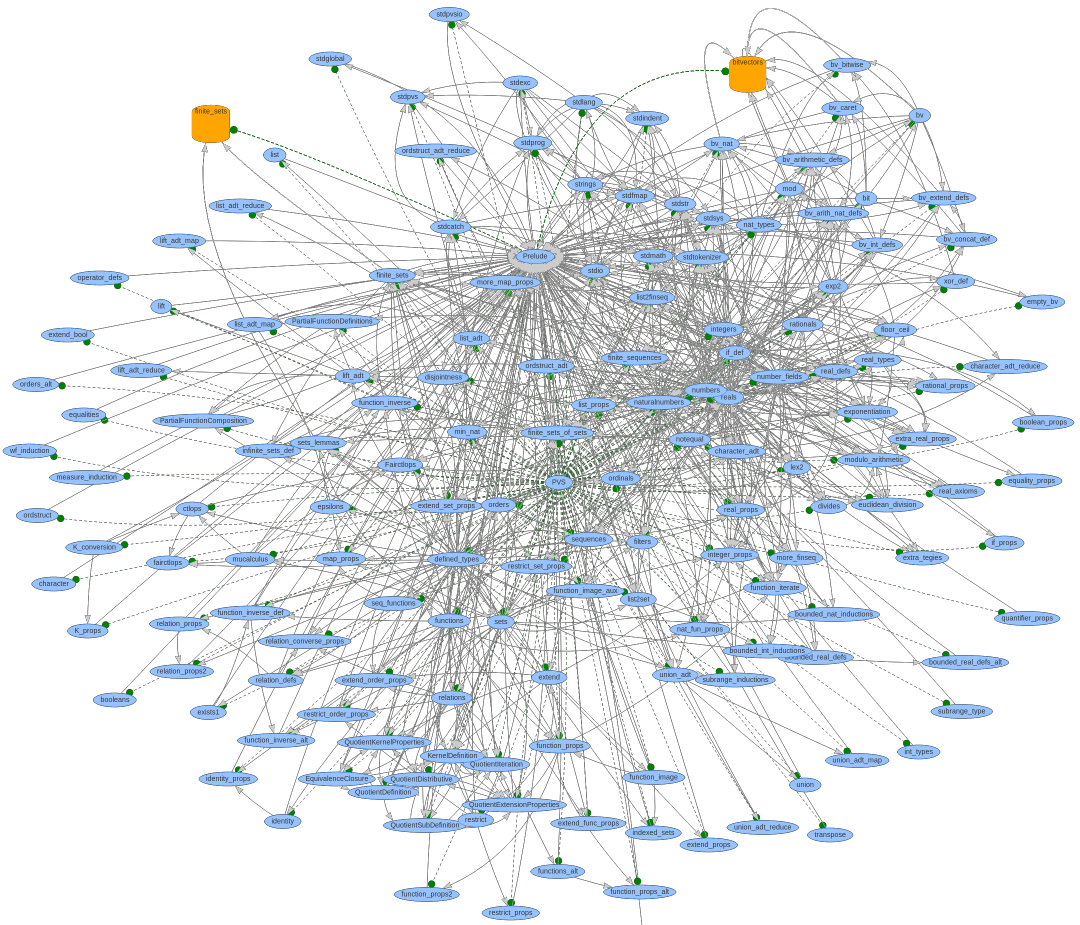
\includegraphics[width=10cm]{img/pvs-full-graph}}\hspace*{-5.35cm}\vspace*{-2cm}
  \fbox{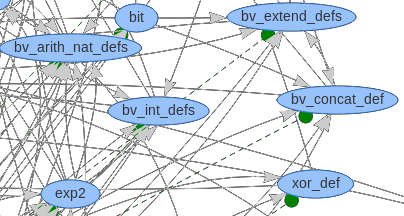
\includegraphics[width=5cm]{img/pvs-graph-detail}}\vspace*{2cm}
\caption{The Basic PVS Libraries in the \mathhub Theory Graph Viewer}\label{fig:graph}
\end{figure}

PVS libraries make heavy use of theories as a structuring mechanism, which makes a graph
viewer for PVS particularly attractive.
\autoref{fig:graph} shows the full graph in a central-gravity layout
induced by the PVS prelude, where we have (manually) clustered the subgraphs for bit vectors and finite sets (the orange barrel-shaped nodes).
The lower right corner shows a zoomed-in fragment.

The theory graph allows dragging nodes around to fine-tune the layout.  Hovering over a
node or edge triggers a preview of the theory.
All nodes support the same context menu actions
in the graph viewer as the corresponding theories do in the browser above.
Thus, it is possible to select a theory in the graph viewer and
then navigate to it in the browser or (if run locally) in the PVS system.

\subsection{Search}

\mws \cite{mathwebsearch} is an \ommt-level formula search engine that uses query
variables for subterms and first-order unification as the query language.  It is developed
independently, but \mmt includes a plugin for generating \mws index files using its
content MathML interface.  Thus, any library available to \mmt can be indexed and searched
via \mws.  Moreover, \mmt includes a frontend for \mws so that search queries can be
supplied in any format that \mmt can understand, e.g., the XML format produced by PVS.

\begin{figure}[ht]\centering
\begin{lstlisting}[language=XML]
<mws:query limitmin="0" answsize="1000" totalreq="yes"
  output="xml" xmlns:m="http://www.w3.org/1998/Math/MathML"
  xmlns:mws="http://www.mathweb.org/mws/ns">
 <mws:expr>
  <apply>
   <csymbol>http://cds.omdoc.org/urtheories?LambdaPi?apply</csymbol>
   <csymbol>http://pvs.csl.sri.com/?PVS?pvsapply</csymbol>
   <mws:qvar xmlns:mws="http://www.mathweb.org/mws/ns">I1</mws:qvar>
   <mws:qvar xmlns:mws="http://www.mathweb.org/mws/ns">I2</mws:qvar>
   <csymbol>http://pvs.csl.sri.com/prelude?EquivalenceClosure?EquivClos</csymbol>
   <mws:qvar xmlns:mws="http://www.mathweb.org/mws/ns">A</mws:qvar>
  </apply>
 </mws:expr>
</mws:query>
\end{lstlisting}
\caption{A Query for Applications of EquivClos}\label{fig:pvsquery}
\end{figure}
\mmt exposes the search frontend both in its GUI for humans and as an HTTP service for
other systems.  Here we use the latter: We have added a feature to the PVS
emacs interface that allows users to enter a search query in PVS syntax.  PVS parses the
query, type-checks it, and converts it to XML.  The XML is sent to \mmt, which acts as the
mediator between the proof assistant --- here PVS --- and library management periphery --- here
\mws --- and returns the search results to PVS.

\begin{figure}[ht]\centering
\begin{lstlisting}[language=XML,mathescape]
[ {"lib_name" : "",
   "theory_name" : "EquivalenceClosure",
   "name" : "EquivClosMonotone",
   "Position" : "3_2_5_5_5_5"}, 
  {"lib_name" : "",
   "theory_name" : "EquivalenceClosure",
   "name" : "EquivalenceCharacterization",
   "Position" : "2_2_5_5_5_5"},
  $\ldots$
] 
\end{lstlisting}
\caption{A Query Result for \autoref{fig:pvsquery}}\label{fig:pvsqueryresult}
\end{figure}
The PVS user enters the PVS query \expr{EquivClos(?A)}, where we have extended the
PVS syntax with query variables like \lstinline|?A|. After \ommt translation, this
becomes the \mws query in \autoref{fig:pvsquery} --- note the additional symbols from LF introduced by the representation in the logical framework.
The representation also introduces unknown meta-variables for the domain and range of the \expr{EquivClos} function, which become the additional query variables \lstinline|I1| and \lstinline|I1|.
\mws returns a JSON record with all results, and we show the first two in \autoref{fig:pvsqueryresult}: two occurrences
of (instances of) \expr{EquivClos(?A)} in two declarations in the theory
\expr{EquivalenceClosure} \autoref{fig:intro:prel:pvs:equivclos}.
The attribute \lstinline|lib_name| is the name of the library; by PVS convention, it is empty for the Prelude.
The attributes \lstinline|theory_name| and \lstinline|name| give the declaration that contains the match, and \lstinline|Position| gives the path to its subterm that matched the query.
%There are actually two more
%occurrences in the Prelude which currently require a separate \mws query due to theory
%parameters.

\begin{figure}[ht]\centering
  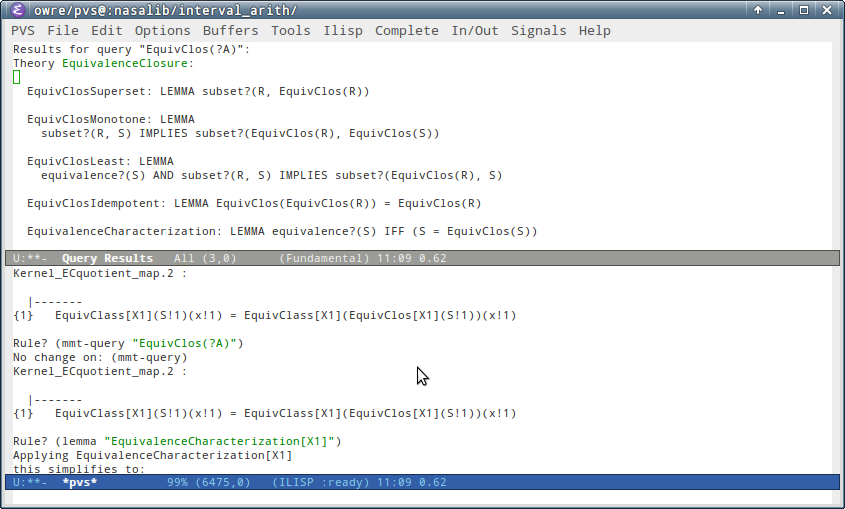
\includegraphics[width=\textwidth]{img/pvs-screenshot2}
\caption{Example for Displaying the Query Result in PVS}\label{fig:pvsprover}
\end{figure}

\autoref{fig:pvsprover} shows what the query will look like while doing a PVS proof.
The current implementation is just a proof-of-concept --- for the mature version the part of PVS that sends the query to the \mmt server and displays the results still has to be implemented thoroughly.
But the remaining steps are straightforward.
%\ednote{@SO: I've rephrased this to look less weak, but it's still weak. Can we strengthen it by promising something like ``the remaining steps will be implemented in a few days''?}

Future work could potentially exploit this functionality to search specifically for existing theorems that may be helpful in a specific part of an ongoing PVS proof.

\subsection{Querying Across Libraries}\label{sec:ulo}
Going beyond a single system, we exported relational data for several theorem prover libraries as RDF triples for more advanced queries without relying on the \mmt system (as published in \cite{ConKohMue:rdaml19}). This relational data is already contained in the underlying \omdoc representation of \mmt archives and can thus be easily generated from imported libraries. In conjunction with alignments (which we will discuss in \autoref{sec:crosslib:alignments}) this allows for conveniently querying for mathematical concepts across different theorem prover libraries using an arbitrary triple store as backend. For example, for the cited paper I set up an instance of Virtuoso Open-Source\footnote{\url{https://github.com/openlink/virtuoso-opensource}}, providing a SPARQL endpoint. Using the query
\begin{lstlisting}
SELECT ?x ?y WHERE {
  ?x ulo:inductive-on ?y .
  http://mathhub.info/MitM/Foundation?NatLiterals?nat_lit ulo:aligned-with ?y . }
\end{lstlisting}
we receive as results (which are shown in \autoref{fig:import:rdfquery}) all functions and predicates defined by induction on the natural numbers regardless of implementation - by only considering those symbols that are aligned with the Math-in-the-Middle symbol for the type of natural numbers.
\begin{figure}[t]\centering
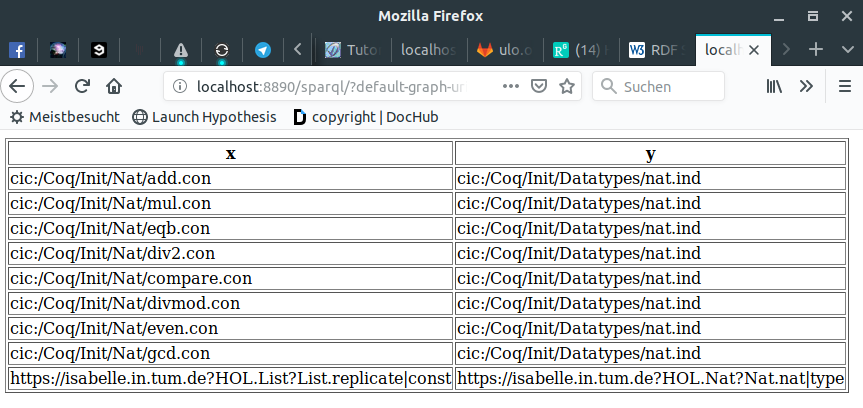
\includegraphics[width=\textwidth]{img/queryresult}
\caption{Virtuoso Output for the Example Query using Alignments}\label{fig:import:rdfquery}
\end{figure}


%%% Local Variables:
%%% mode: latex
%%% TeX-master: "paper"
%%% End:

%  LocalWords:  sec:appl ommt mathhub IanJucKoh:sdm14,MathHub:on visjs visualization fbox
%  LocalWords:  visjs:on fig:graph centering includegraphics hspace vspace compactitem
%  LocalWords:  formalizations MathHub:on mmtpvs:git inparaenum mws emph mathwebsearch
%  LocalWords:  synchronized fig:screenshot1 subterms lstlisting mws:query limitmin ldots
%  LocalWords:  answsize totalreq xmlns:m xmlns:mws mws:expr csymbol mws:qvar EquivClos
%  LocalWords:  fig:pvsquery XML,mathescape EquivalenceCharacterization lstinline omdoc
%  LocalWords:  fig:pvsqueryresult fig:pvsequivclos pvs-screenshot fig:pvsprover
%  LocalWords:  textwidth
